\documentclass[10pt,a4paper]{article}
\usepackage[latin1]{inputenc}
\usepackage{amsmath}
\usepackage{amsfonts}
\usepackage{amssymb}
\usepackage{graphicx}
\usepackage{graphics}

\begin{document}

%\begin{table}[ht]
%\begin{minipage}[b]{.7\textwidth}
{\centering
{\tiny
\begin{tabular}{ccc}
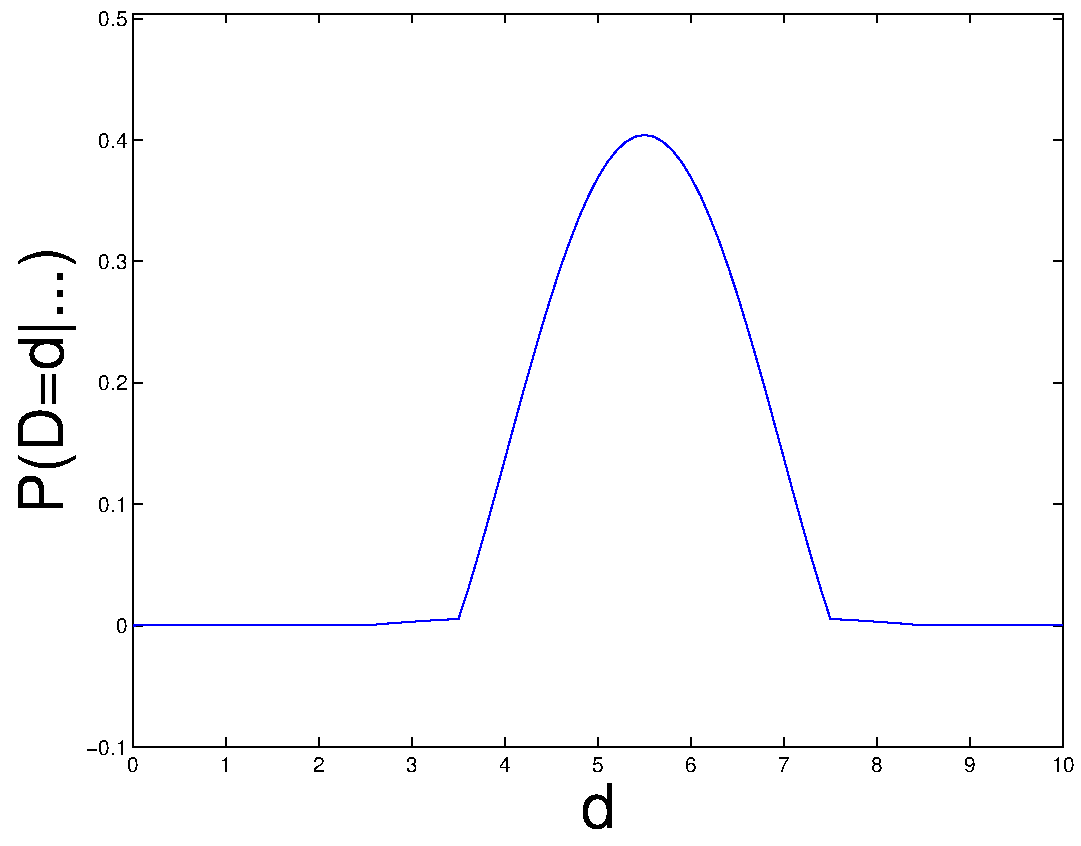
\includegraphics[width=90pt]{r1.pdf} & 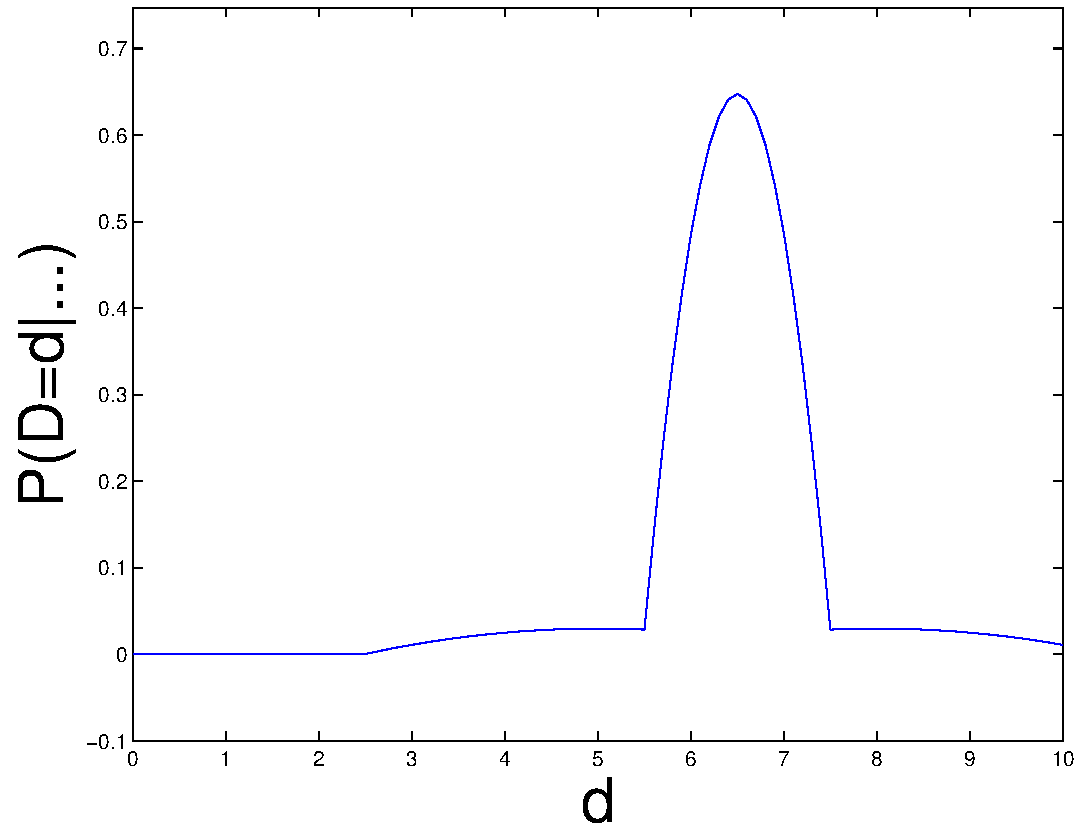
\includegraphics[width=90pt]{r2.pdf} & 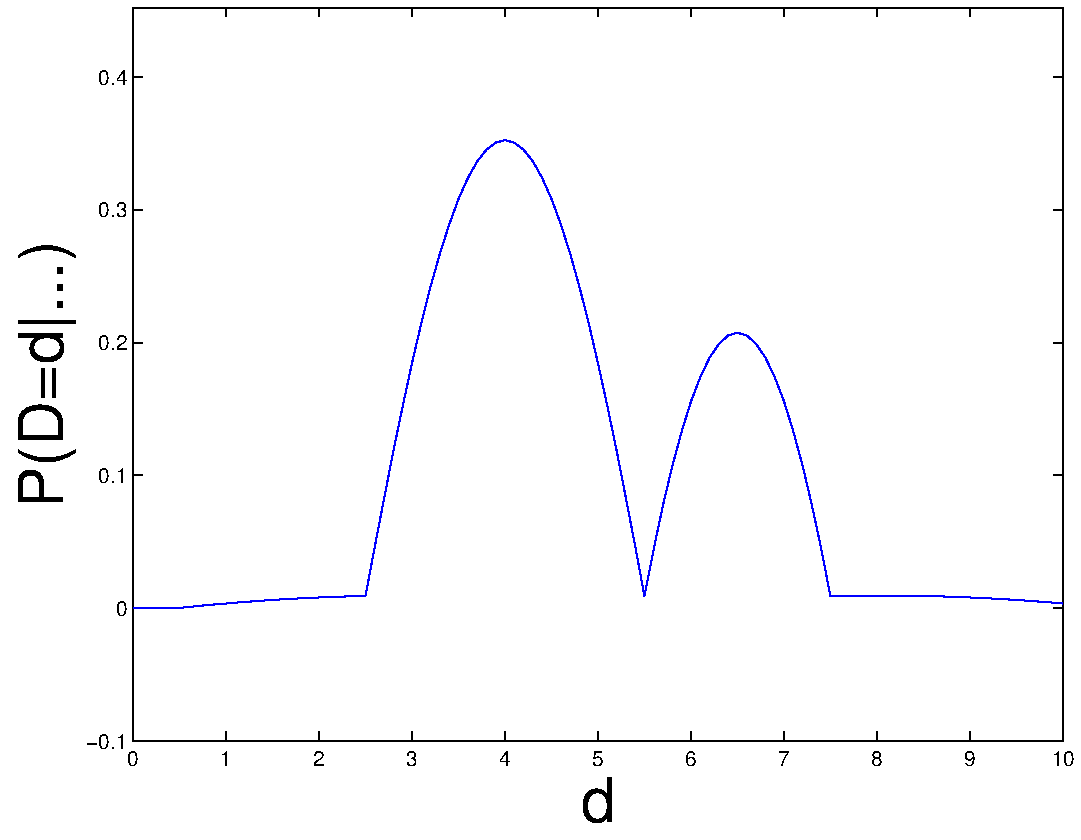
\includegraphics[width=90pt]{r3.pdf} \\  
{\small$\mathbf{E}(d|x1=5) = 4.98$} & {\small$\mathbf{E}(d|x1=5,x2=8)= 6.0$} & {\small$\mathbf{E}(d|x1=5,x2=8,x3=3) = 4.39$}\\
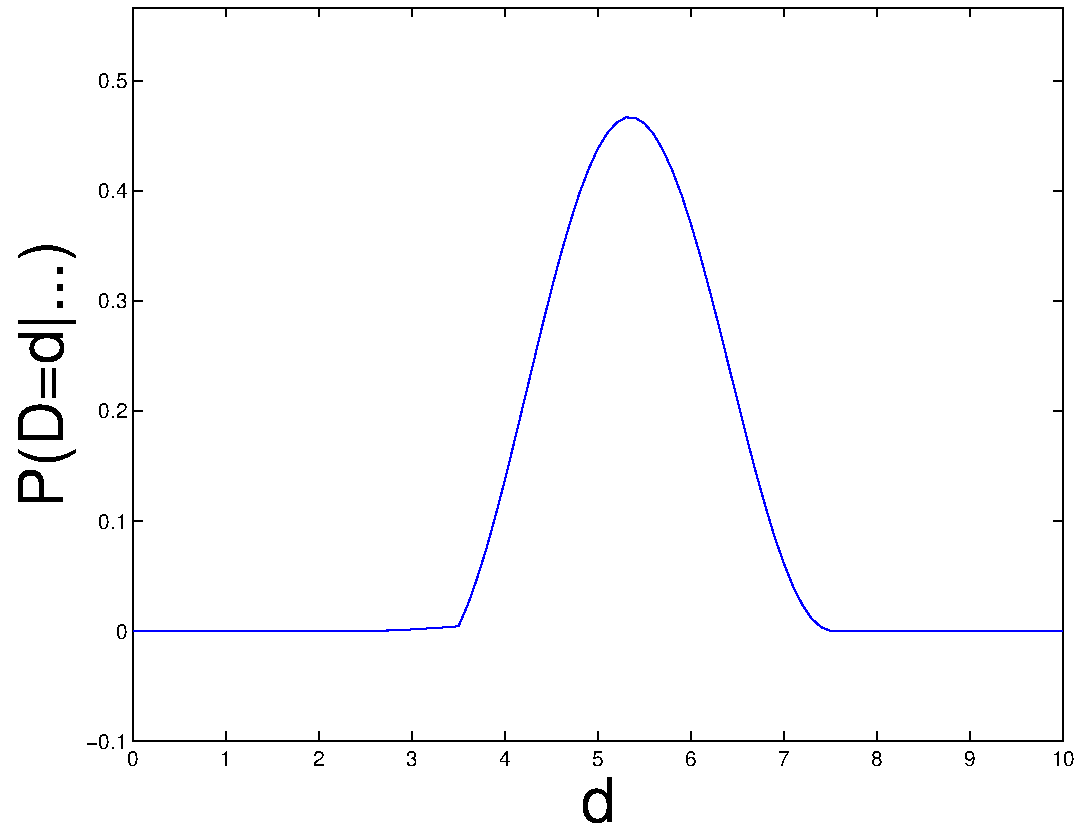
\includegraphics[width=90pt]{r4.pdf} & 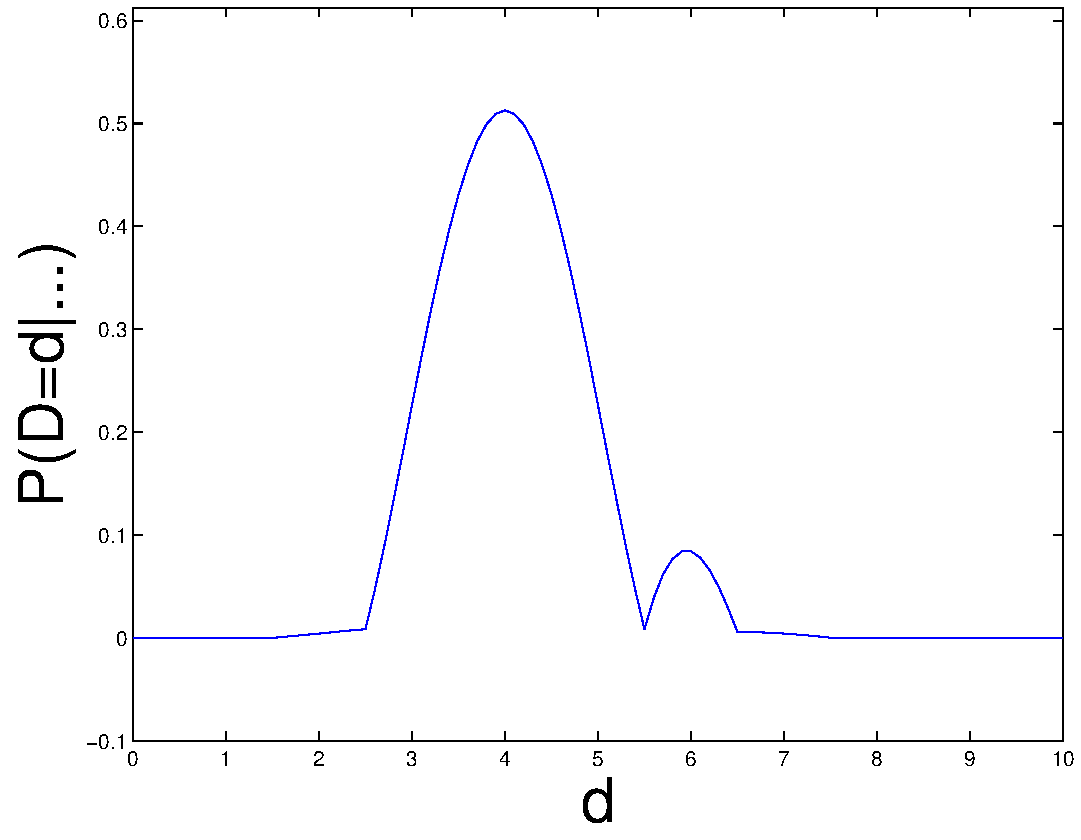
\includegraphics[width=90pt]{r5.pdf} & 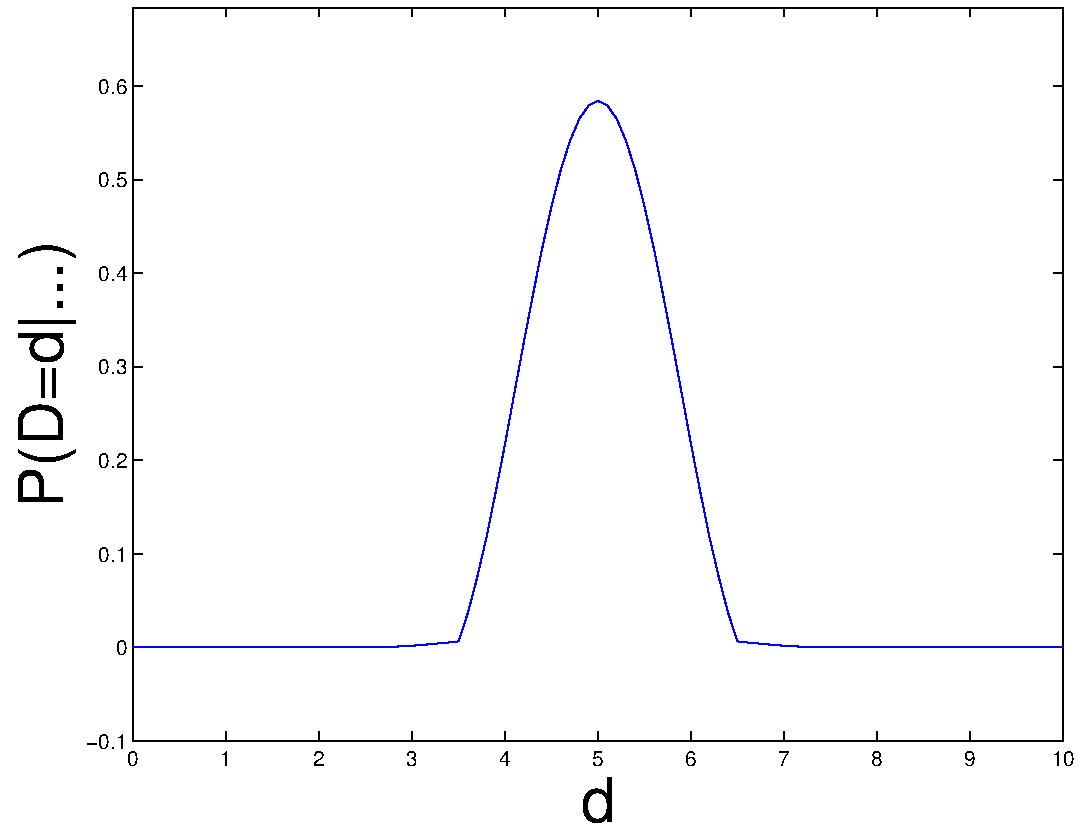
\includegraphics[width=90pt]{r6.pdf} \\
{\small$\mathbf{E}(d|x1=5,x2=5) = 4.98$} & {\small$\mathbf{E}(d|x1=5,x2=5,x3=6) = 5.45$} & {\small$\mathbf{E}(d|x1=4,x2=6) = 4.89$} 
\end{tabular}
}
}
\begin{tabular}{cc}
\hline
{\small$p(d|x1=5), \mathbf{E}(d) = 4.98$} & {\small$p(d|x1=5,x2=8), \mathbf{E}(d) = 6.0$} \\
{\small$p(d|x1=5,x2=8,x3=3), \mathbf{E}(d) = 4.39$} & {\small$p(d|x1=5,x2=5), \mathbf{E}(d) = 4.98$} \\ {\small$p(d|x1=5,x2=5,x3=6), \mathbf{E}(d) = 5.45$} & {\small$p(d|x1=4,x2=6), \mathbf{E}(d) = 4.89$} \\
\hline
\end{tabular}



{\centering
\begin{tabular}{l}
\includegraphics[width=250pt]{o1_x1b1.ps} \\
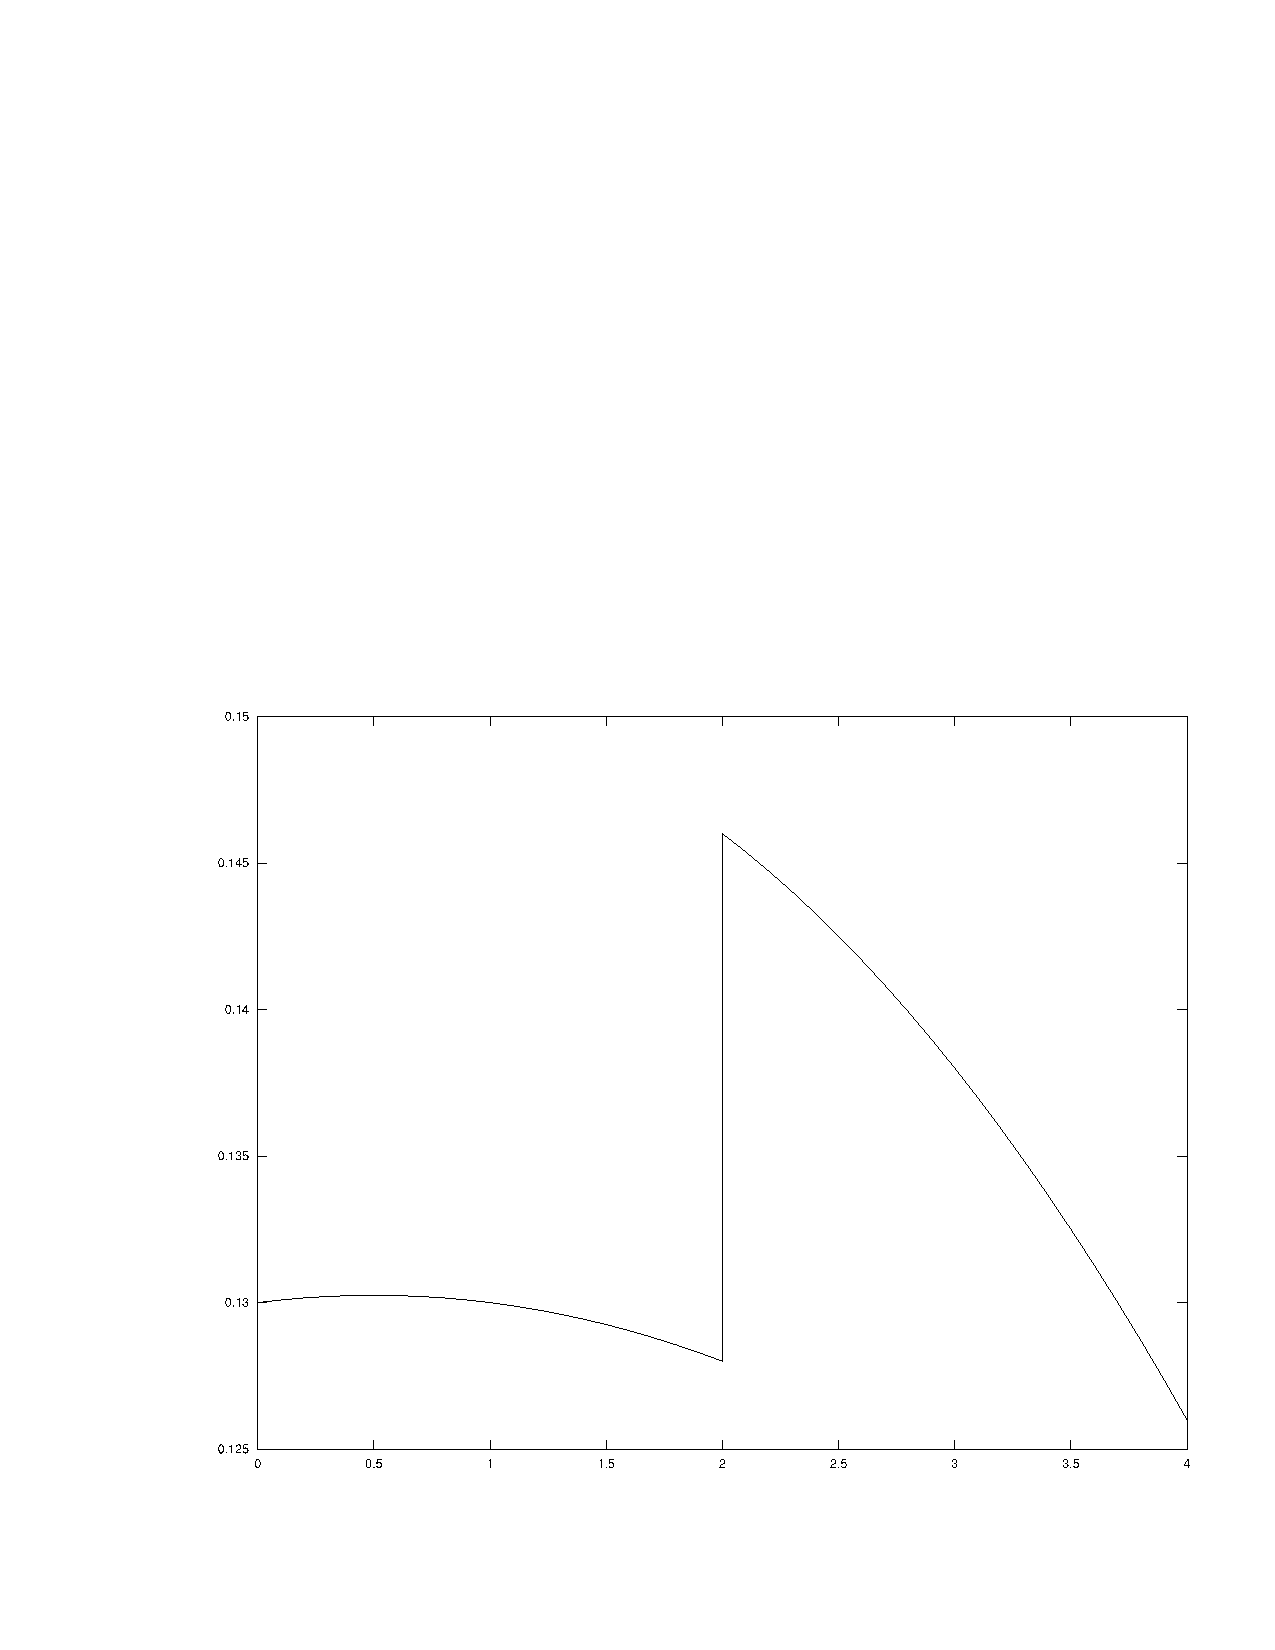
\includegraphics[width=100pt]{o1_b1false.pdf} \\
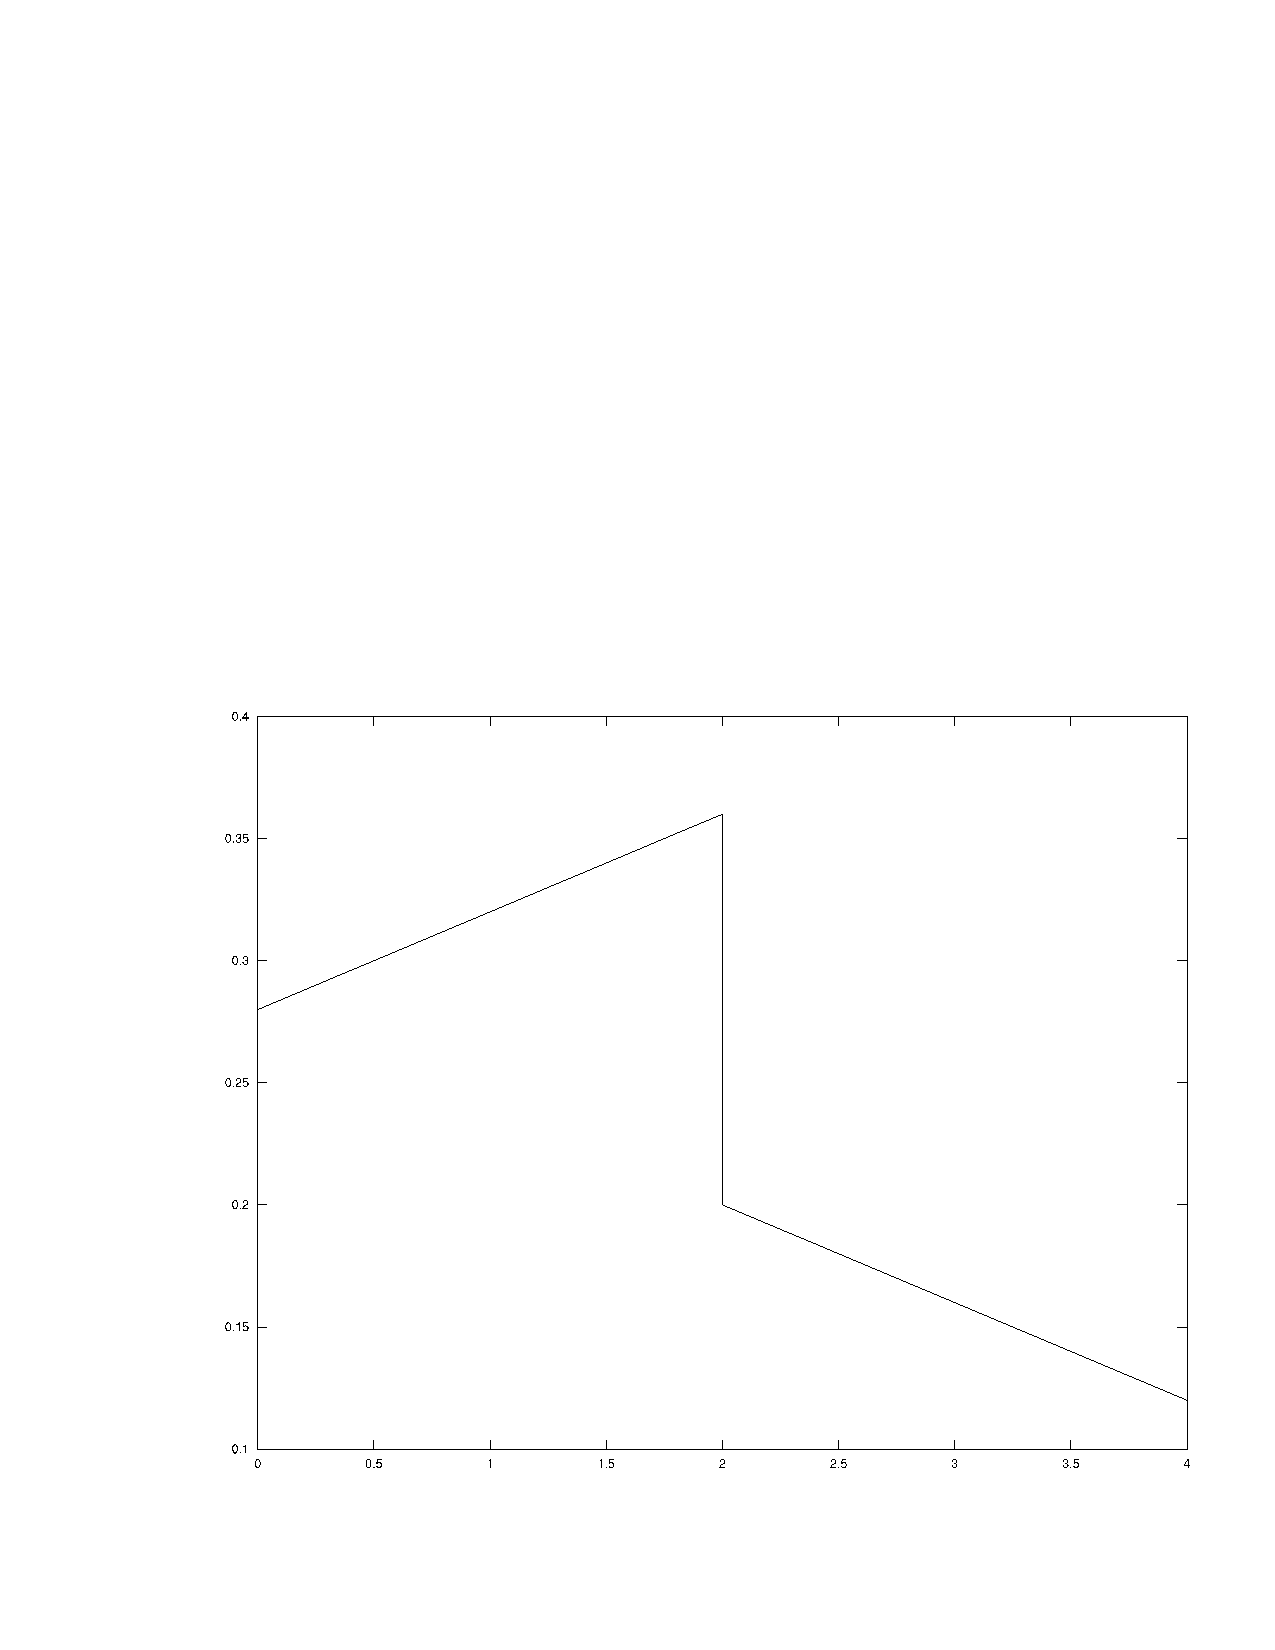
\includegraphics[width=100pt]{o1_b1true.pdf} \\
\end{tabular}
}

{\centering
\begin{tabular}{ccc}
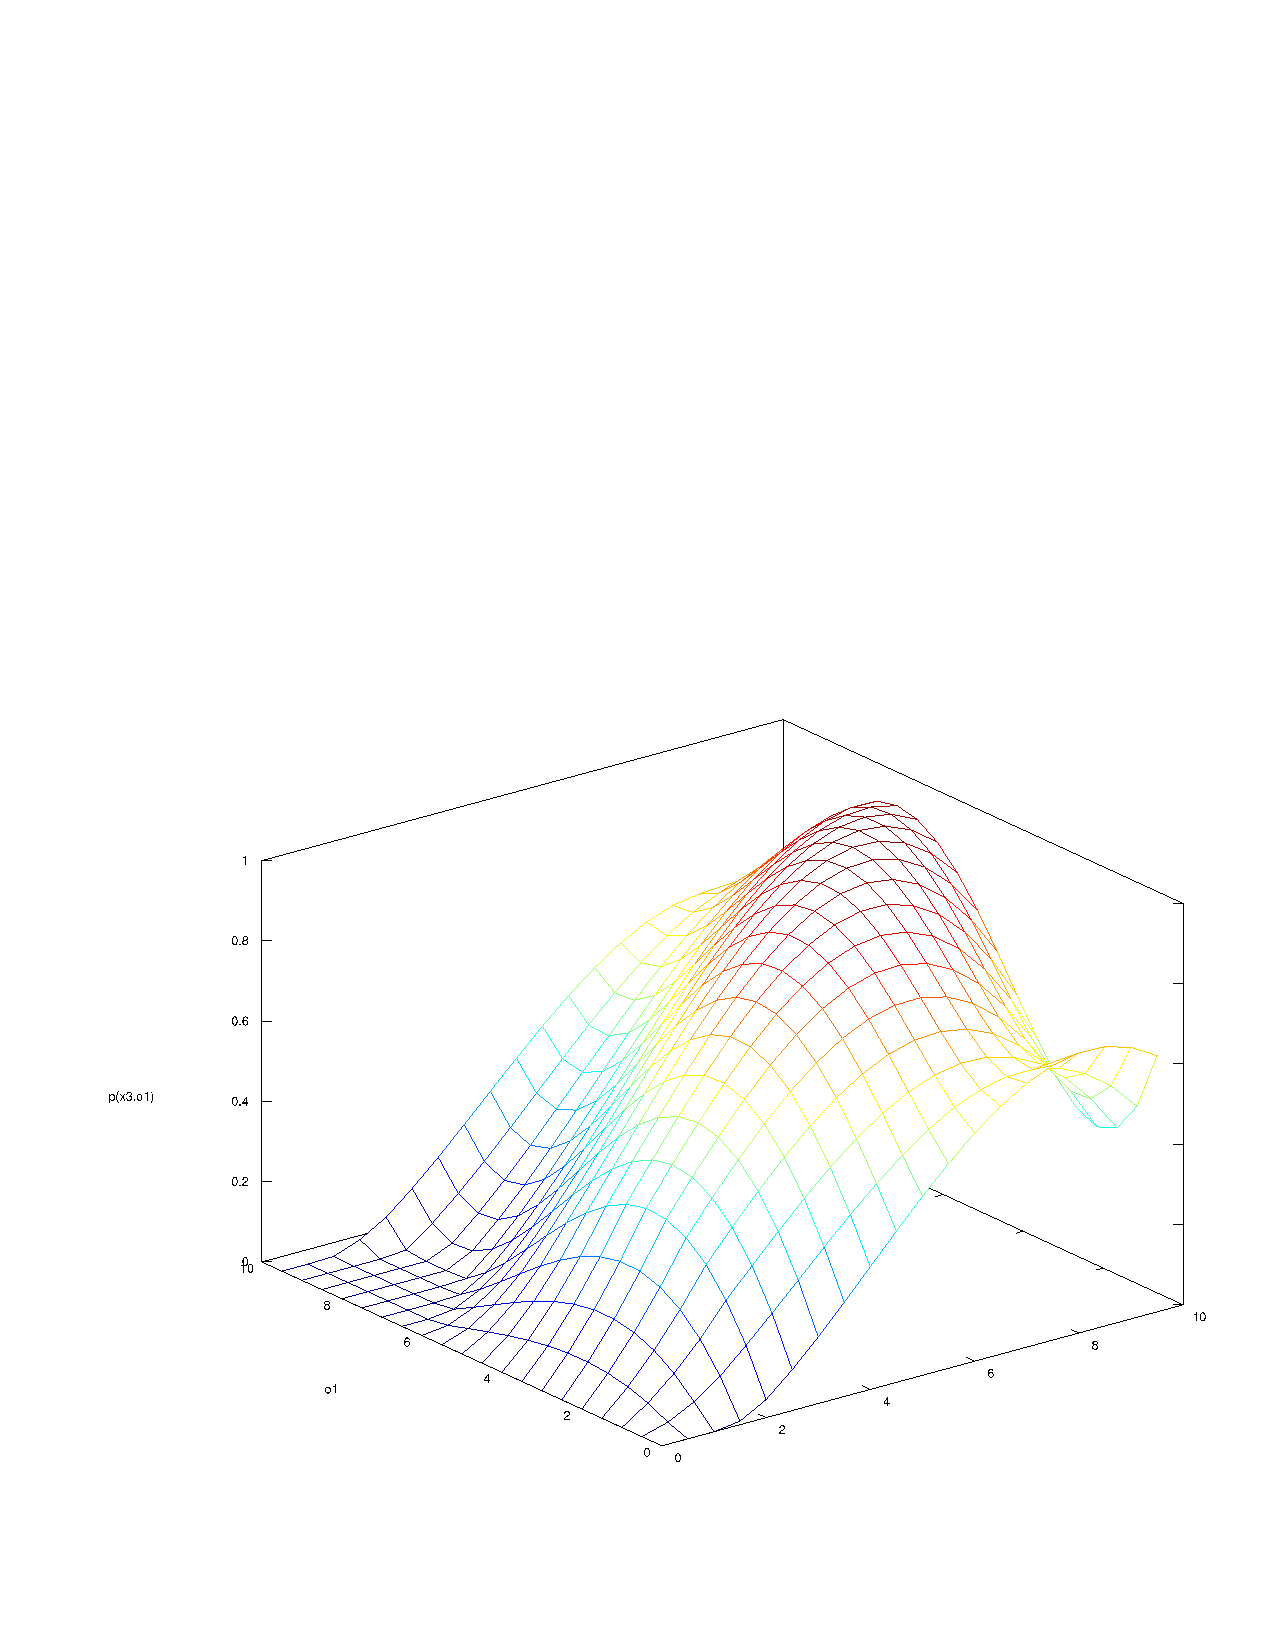
\includegraphics[width=100pt]{tracker_3d_x3o1.pdf} & 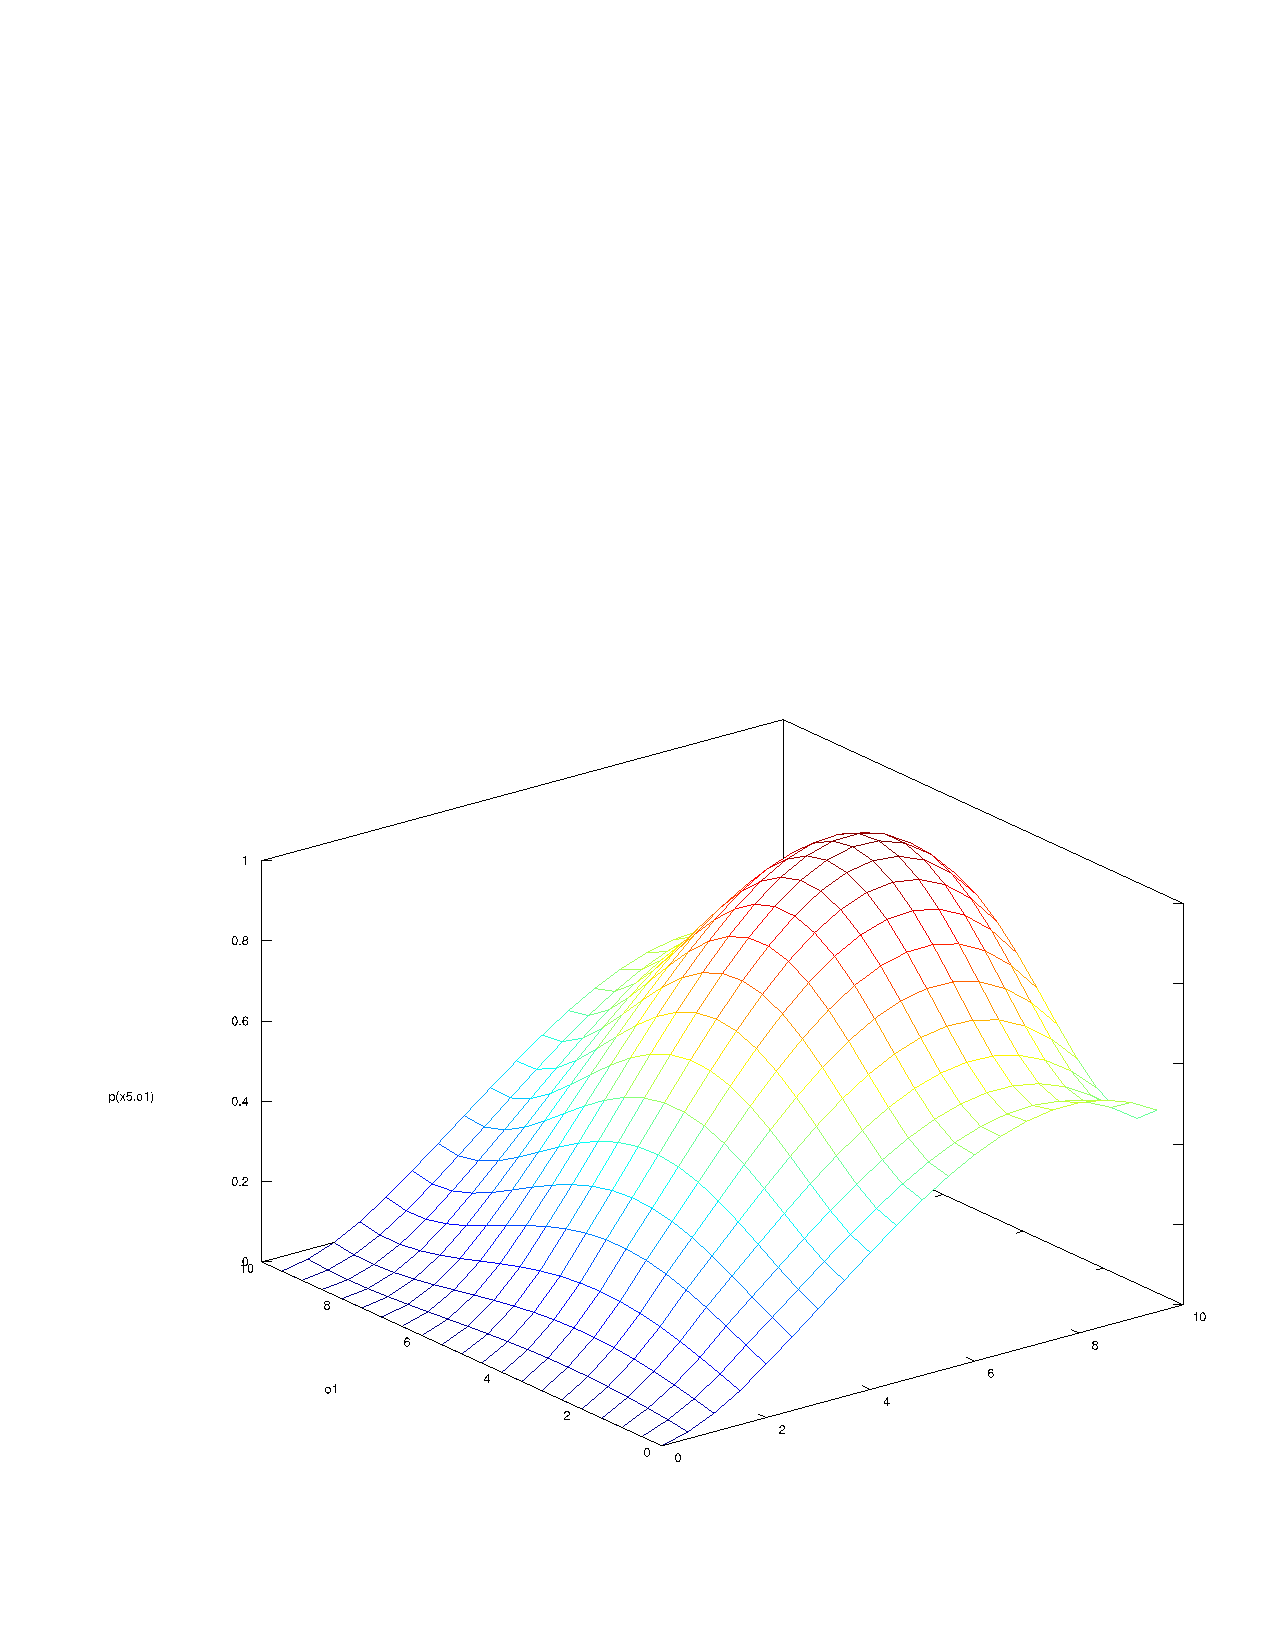
\includegraphics[width=100pt]{tracker_3d_x5o1.pdf} & 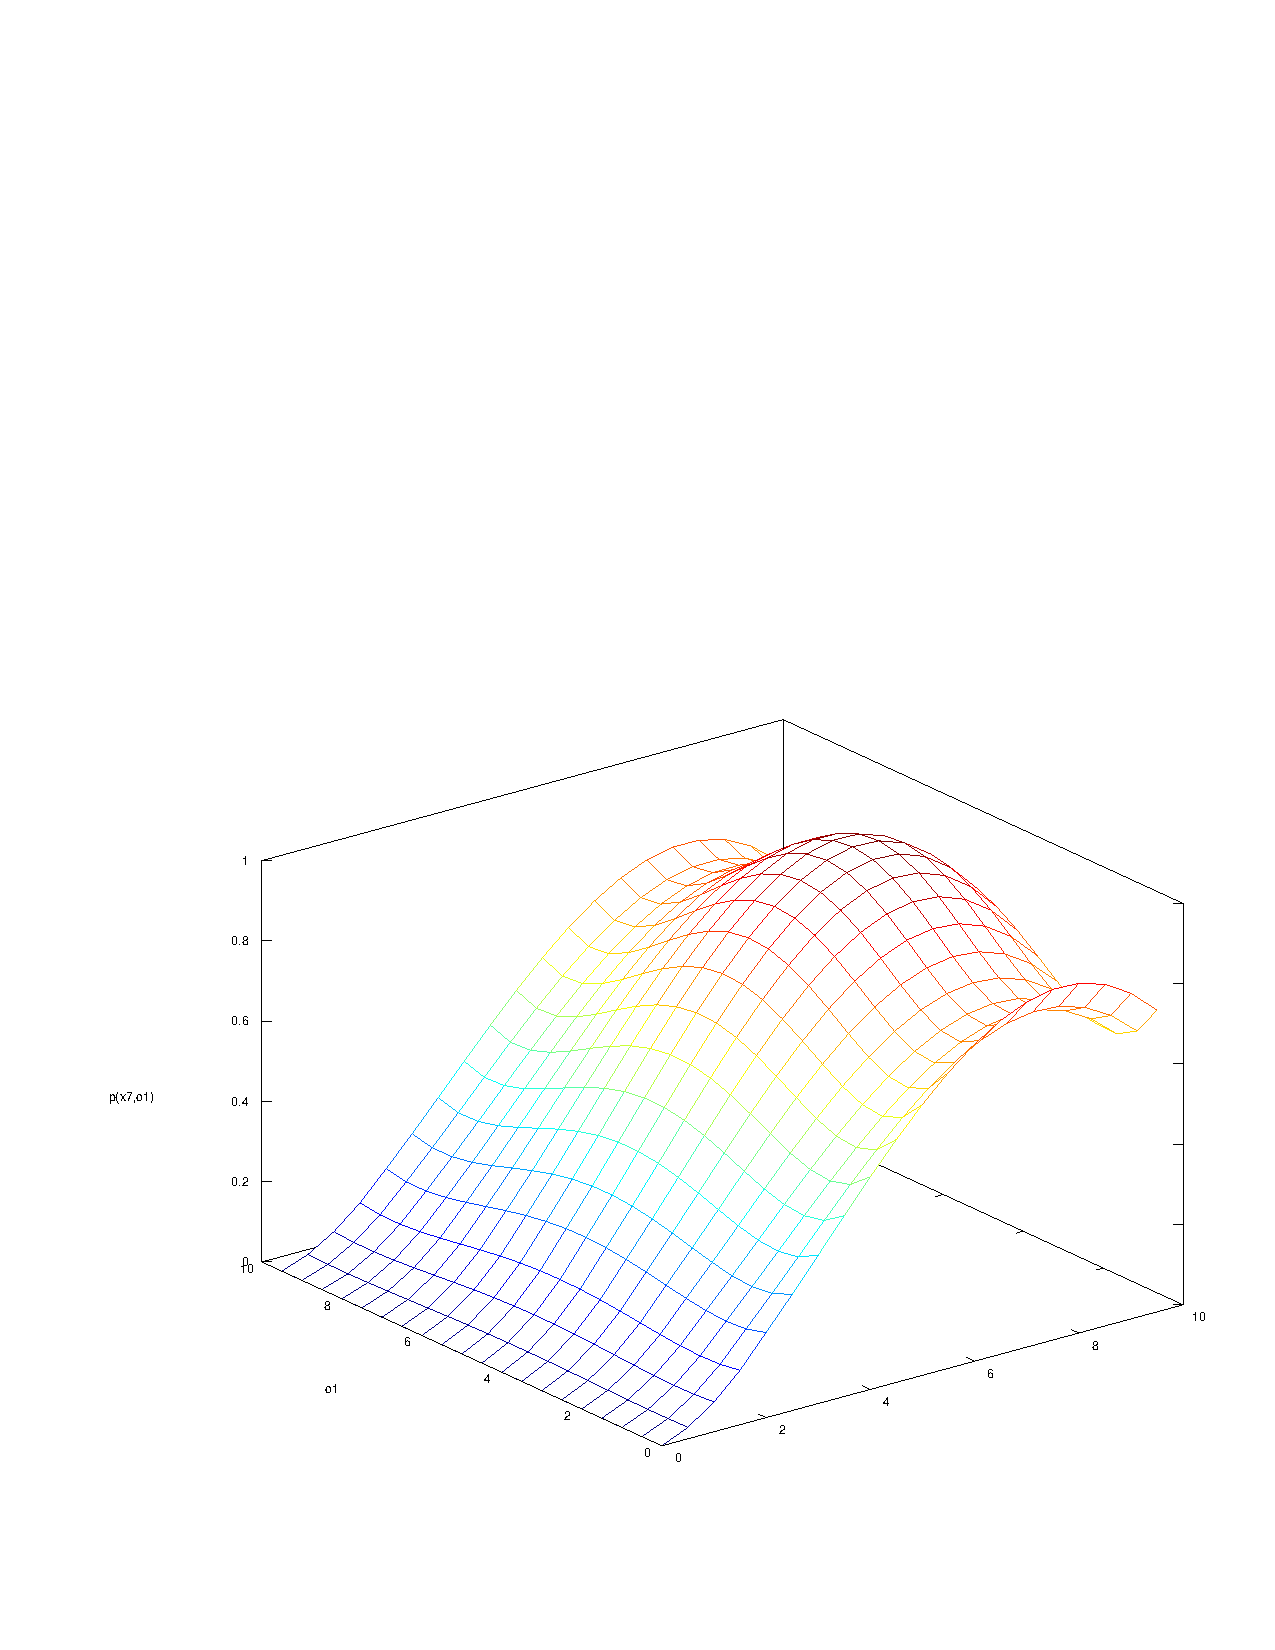
\includegraphics[width=100pt]{tracker_3d_x7o1.pdf} \\
(a) & (b) & (c) \\
\multicolumn{3}{c}{The value of $p(x3,o1)$, $p(x5,o1)$ and $p(x7,o1)$}
\end{tabular}
}
%\end{minipage}

%\begin{minipage}[b]{0.5\linewidth}

%\end{minipage}

%\end{table}

%\begin{figure}
%\includegraphics[width=120pt]{o1_b1_false.ps}
%\end{figure}

\end{document}